\section{Phi Nodes}

In SSA IR, we encountered the issue of figuring out which variable version to use after a join point where multiple paths were coming in with different versions of the same variable. As a solution to this, phi nodes or phi functions are extremely helpful that could be placed only at the beginning of a basic block with multiple edges coming in (join point).

These phi nodes can be placed at each join point for every variable in the program. This placement strategy is a bit wasteful as illustrated in the following diagram:

\begin{figure}[htp]
\centering
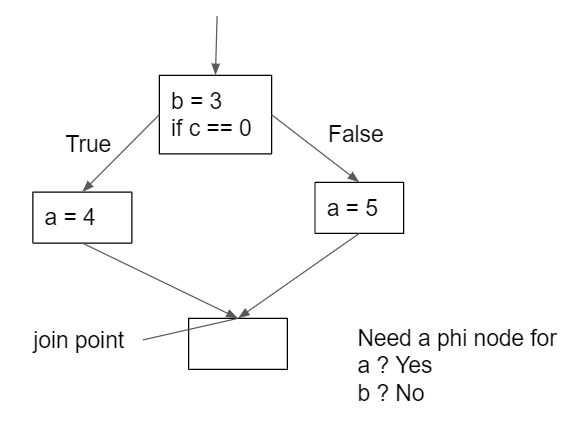
\includegraphics[height=6cm]{images/phinodes.png}
\caption{Placement of \(\Phi\) nodes}
\end{figure}

\subsection{Path Convergence Criterion}

Consider z to be node with multiple edges coming in (thus it is a join point). We need \(\Phi\) node for variable a at node z if and only if
\begin{enumerate}
    \item There is a block x containing the definition of a.
    \item There is a block y (not x) containing the definition of a.
    \item There are non empty paths \(P_{xz}\) and \(P_{yz}\) from x to z and y to z respectively.
            \begin{figure}[htp]
\centering
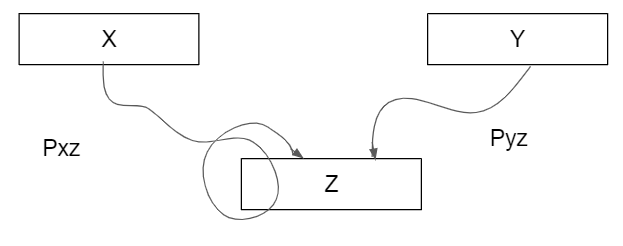
\includegraphics[height=3cm]{images/Condition123.png}
\caption{CFG for condition 1, 2, 3}
\end{figure}
    \item \(P_{xz}\) and \(P_{yz}\) should not have any node in common except z.
        \begin{figure}[htp]
\centering
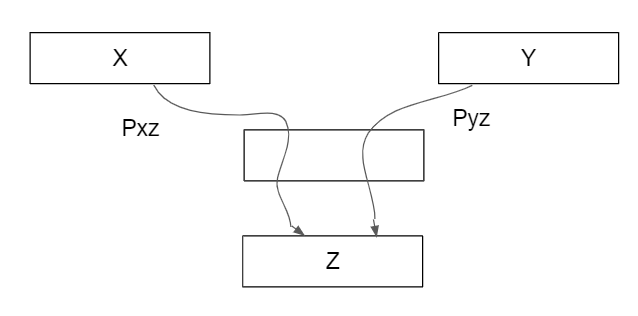
\includegraphics[height=3cm]{images/Condtion4.png}
\caption{Violation of Condition 4}
\end{figure}
    \item The node z does not appear within both  \(P_{xz}\) and \(P_{yz}\), prior to the end. It is fine if z appears only in one of the path before end.
            \begin{figure}[htp]
\centering
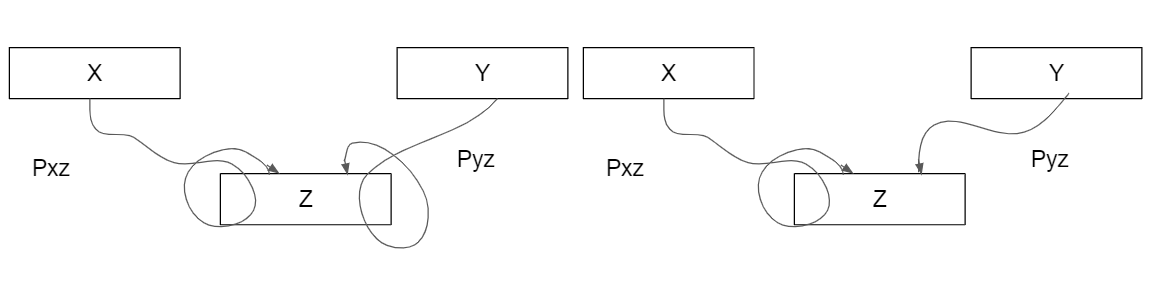
\includegraphics[height=3cm]{images/Condition5.png}
\caption{Cpndition 5: Left CFG does not need \(\Phi\) node, right CFG needs \(\Phi\) node}
\end{figure}
\end{enumerate}

\subsection{Iterative Fixed Point Algorithm}

while \{there are nodes x, y, z satisfying condition 1-5 and z does not contain a \(\Phi\) node for a\}\\
do \{insert \(a \leftarrow \Phi(a_1, a_2, ..., a_j)\) \}

The \(\Phi\) function has as many 'a' arguments as there are predecessors of z. Since the conditions 1-5 are both sufficient and necessary, the above algorithm is sound and complete.
